\documentclass{book}
\usepackage{latexsym}
\usepackage{amsmath}
\usepackage{bm}
%%%%%%%%%%%%%%%%%%%%force formula number size unchanged
\makeatletter
\def\my@tag@font{\normalsize}
\def\maketag@@@#1{\hbox{\m@th\normalfont\my@tag@font#1}}
\let\amsmath@eqref\eqref
\renewcommand\eqref[1]{{\let\my@tag@font\relax\amsmath@eqref{#1}}}
\makeatother
\usepackage{amssymb}
\usepackage{color}
%%%%%%%%%%%%%%%%%%%%%%%%%%set table background color
\usepackage{colortbl}
\definecolor{mygray}{gray}{.9}
\definecolor{mypink}{rgb}{.99,.91,.95}
\definecolor{mycyan}{cmyk}{.3,0,0,0}
%\rowcolor{mygray} k&	50&	100&	200&	500 &800	&1000&	1100&	1200\\
%%%%%%%%%%%%%%%%%%%%%%%%%
\usepackage{mathrsfs}  %special symbol package

\topmargin=-0.5truein \oddsidemargin=0.25truein
\evensidemargin=0.25truein \textwidth=6truein \textheight=9truein
\usepackage[paperwidth=21cm,paperheight=29.7cm]{geometry}
\geometry{verbose,tmargin=2.3cm,bmargin=3.4cm,lmargin=1.5cm,rmargin=1.5cm,headheight=1.25cm,footskip=1.25cm}
%%%%%%%%%%%%%%%%%%%%%%%%use upper and lower margin values for line break header
%\geometry{verbose,tmargin=1.75cm,bmargin=3.95cm,lmargin=1.5cm,rmargin=1.5cm,headheight=1.25cm,footskip=1.25cm}
\usepackage[labelsep=period, labelfont=bf, aboveskip=10pt, belowskip=2pt, font=small, font=it]{caption}

\usepackage[ngerman]{babel}
\uchyph=0
\tolerance=1
\emergencystretch=\maxdimen
\hyphenpenalty=10000
\hbadness=10000
%%%%%%%%%

\usepackage{indentfirst} %Indent the first line of a paragraph
\parindent=10pt
\linespread{1.0}
\setlength{\parskip}{0pt}

\usepackage{ifthen}
%ifthen
%\ifthenelse
%\\whiledo
\usepackage{amsmath}
\usepackage{fancyhdr}
\usepackage{amsthm}
\usepackage[normalem]{ulem}

%%%%%%%%%%%%%%%%%%%%%%%%%%%%%%%%%%%%%%%%%%%%%%%%%%%%%%%%%%%%??????
\usepackage[latin1]{inputenc}
\usepackage{amsfonts}
\usepackage{amssymb}
%\usepackage{multicol,lipsum} % for two columns
%\usepackage{blindtext} % for two columns
\usepackage{multicol}
\usepackage{makeidx}
\usepackage{graphicx}
\usepackage{ulem} % is used for different types of under lining
\usepackage{subcaption}
\usepackage[numbers,sort&compress]{natbib}
\usepackage{setspace}
%%%%%%%%%%%%%%%%%%%%%%%%%%%%%%%%%%%%%%%%%%%%%%%%%%%%%%%%%%%%%%

\fancyhead{}%
\fancyfoot{}%
\pagestyle{fancy}
\fancyhead[L]{\ifthenelse{\value{page}=1}{first page}{second page}}
\pagestyle{fancy}
\addtolength{\headheight}{\baselineskip}
\fancyhf{}


\fancyhead[OR, EL]{\fontsize{9pt}{12pt}\small\thepage\\\vspace{1pt}}
\fancyhead[EC]{\fontsize{9pt}{12pt}{\small{{Authors Name1 \textit{et al.}}:~~Paper Title}}\\}
% Single page header
\fancyhead[OC] {\fontsize{9pt}{12pt}{\small{Journal Title 2025; X(X): XX-XX}}\\}
% Double page header
\fancypagestyle{plain}{\renewcommand{\headrulewidth}{0pt}\fancyhf{}}

\renewcommand{\headrulewidth}{0pt}% header line width is zero, go to header line
\renewcommand{\footrulewidth}{0pt}% the footnote line width is zero, go to the footnote line

\voffset=0cm
\headsep=0.5cm
\footskip=1cm

\usepackage{titlesec}
\setcounter{secnumdepth}{4}
\renewcommand\thesection{\arabic{section}} %title number 01 becomes 1
\titlelabel{\thetitle.~~}
\titlespacing*{\subsubsection}{0pt}{12pt}{0pt}
\titleformat{\subsection}{\bfseries\slshape}{\thesubsection.}{0.5em}{}
\titleformat{\subsubsection}{\bfseries\slshape}{\thesubsubsection.}{0.5em}{}

\setlength{\columnsep}{1.5em} %set column spacing
\setlength{\columnseprule}{12.5em} %set the column width of the column
%%%%%%%%%%%%%%%%%%%

\usepackage{times}
\usepackage{calc}
\usepackage{xcolor}
\usepackage{amsmath}
\usepackage{amssymb}
\usepackage{array}
\usepackage{booktabs}
\usepackage{caption}
\usepackage{longtable}
\usepackage{tabularx}
\usepackage{fancyvrb}
\usepackage{graphicx}
\usepackage{epstopdf}
\usepackage{ifthen}
\usepackage{paralist}
%%%%%%%%%\usepackage{paralist}
\let\enditemize\endcompactitem
\let\enumerate\compactenum
\let\endenumerate\endcompactenum
\let\description\compactdesc
\let\enddescription\endcompactdesc
%%%%%%%%%%%%%%%%%%%%
\usepackage{titletoc}
\usepackage{ulem}
\usepackage{float}
\usepackage{latexsym}

\usepackage{dsfont}
\usepackage{makeidx}
\usepackage{lipsum}
\usepackage{imakeidx}
\usepackage{multirow}

\usepackage[hang]{footmisc} %make footnotes indent a fixed width
\renewcommand{\footnoterule}{\vspace*{1pt}\hrule width 0.4pt\columnwidth height 0.4pt \vspace*{3pt}}
\footnotemargin=0.5em

%%%%%%%%%%%%%%%%%%%%%%%%%%%%%%%%%%%%%%%%%%%%%%%%%%%
\makeatletter
\def\thm@space@setup{\thm@preskip=0pt
\thm@postskip=0pt}
\makeatother
\newtheoremstyle{remark}
{} %Aboveskip
{} %Below skip
{\mdseries} %Body font e.g.\mdseries,\bfseries,\scshape,\itshape
{} %Indent
{\bfseries} %Head font e.g.\bfseries,\scshape,\itshape
{.} %Punctuation afer theorem header
{ } %Space after theorem header
{} %Heading
%%%%%%%%%%%%%%%%%%%%%%%%%%%%%%%%%%%%%%%%%%%%%%%%%%%%%%
\theoremstyle{remark}
\newtheorem{theorem}{\it\indent Theorem}[section]
\newtheorem{lemma}{\it\indent Lemma}[section]
\newtheorem{proposition}{\it\indent Proposition}[section]
\newtheorem{remark}{\it\indent Remark}[section]
\newtheorem{example}{\it\indent Example}[section]
\newtheorem{definition}{\it\indent Definition}[section]
%%%%%%%%%%%%%%%%%%%%%%%%%%%%%%%%%%%%%%%%%%%%%%
\makeatletter
\newenvironment{pf}[1][\proofname]{\par
  \pushQED{\qed}%
  \normalfont \topsep0\p@\relax
  \trivlist
  \item[\hskip\labelsep\itshape
  #1\@addpunct{.}]\ignorespaces
}{%
  \popQED\endtrivlist\@endpefalse
}
\makeatother
%%%%%%%%%%%%%%%%%%%%%%%%%%%%%%%%%%%%%%%%%%
%\numberwithin{equation}{section} %change the formula number (1) to (1.1)
%\def\be{\begin{equation}}
%\def\ee{\end{equation}}
%\def\ba{\begin{array}}
%\def\ea{\end{array}}
%\def\benu{\begin{enumerate}}
%\def\eenu{\end{enumerate}}
%\def\bt{\begin{theorem}}
%\def\et{\end{theorem}}
%\def\bl{\begin{lemma}}
%\def\el{\end{lemma}}
%\def\br{\begin{remark}}
%\def\er{\end{remark}}
%\def\bd{\begin{definition}}
%\def\ed{\end{definition}}
%\def\bp{\begin{proposition}}
%\def\ep{\end{proposition}}
%\def\bc{\begin{corollary}}
%\def\ec{\end{corollary}}

\begin{document}
\renewcommand{\qedsymbol}{}
\DeclareFixedFont{\Head}{OT1}{phv}{bx}{n}{18pt}
\DeclareFixedFont{\SEC}{OT1}{phv}{bx}{n}{12pt}
\DeclareFixedFont{\Journal}{OT1}{phv}{bx}{n}{11pt}
\DeclareFixedFont{\Name}{OT1}{ptm}{bx}{n}{12pt}%
\DeclareFixedFont{\Address}{OT1}{ptm}{m}{n}{9pt}
\DeclareFixedFont{\Emailaddress}{OT1}{ptm}{bx}{n}{12pt}
\DeclareFixedFont{\Emailaddresscontent}{OT1}{ptm}{m}{n}{9pt}%
\DeclareFixedFont{\Citation}{OT1}{ptm}{bx}{n}{12pt}
\DeclareFixedFont{\Citationcontent}{OT1}{ptm}{m}{n}{9pt}
\DeclareFixedFont{\Date}{OT1}{ptm}{m}{n}{9pt}
\DeclareFixedFont{\Abstract}{OT1}{ptm}{bx}{n}{12pt}
\DeclareFixedFont{\Abstractcontent}{OT1}{ptm}{m}{n}{10pt}
\DeclareFixedFont{\FirstLevel}{OT1}{ptm}{bx}{n}{14pt}
\DeclareFixedFont{\SecondLevel}{OT1}{ptm}{bx}{it}{10pt}
\DeclareFixedFont{\ThirdLevel}{OT1}{ptm}{bx}{it}{10pt}%
\DeclareFixedFont{\Text}{OT1}{ptm}{m}{n}{10pt}
\DeclareFixedFont{\References}{OT1}{ptm}{bx}{n}{14pt}%
\DeclareFixedFont{\ZJL}{T1}{pxtt}{bx}{n}{12pt}
\chapter*{}
\setcounter{page}{1}%
\vspace{-4.65cm}
%\makebox[48.6em][l]{
\noindent
\begin{tabular}[H]{lr}\toprule [1pt] \vspace{-0.33cm}\\
\hspace{-2mm}\Journal{Journal Title} & \hspace{49mm}\multirow{5}*{
\includegraphics[height=22mm,width=58mm]{SciencePGLOGO.pdf}}\\
\hspace{-2mm}\Address{2025; X(X): XX-XX} &\\
\hspace{-2mm}\Address{http://www.sciencepublishinggroup.com/x/xxx} &\\
\hspace{-2mm}\Address{doi: 10.11648/j.XXXX.2025XXXX.XX} &\\
%\hspace{-2mm}\Address{ISSN: xxxx-xxxx (Print); ISSN: xxxx-xxxx (Online)} \\
\\\bottomrule [2.5pt]
\end{tabular}
%}
\parskip=12pt
\begin{flushleft}
\noindent \Head{Paper Title (SciencePG-Paper-Title)}
\end{flushleft}
\parskip=8pt
\noindent \Name{Authors Name{\bm{$^{1,*}$}}, Authors Name{\bm{$^{1, 2}$}}}
\parskip=8pt


\noindent \Address{$^1$Department / Faculty of University, University, City, Country\\$^2$Department Name of Institute/Organization, Name of Institute/Organization, City, Country}
\vspace{5pt}

\parskip=4pt
\noindent \Emailaddress{Email address:}\\
\noindent \Emailaddresscontent{email1@authorname.com (author name1), email2@authorname.com (author name2)\\$^*$Corresponding author}
%\noindent \Emailaddresscontent{lanyuyanliang@163.com}

\parskip=8pt
\noindent \Citation{To cite this article:}
\begin{flushleft}
\vspace{-0.56cm}
\noindent \Citationcontent{Authors Name. (2025). Paper Title. {\it Journal of XXXXXX, Volume}(Issue), Page Range. DOI Link}
\vspace{-0.3cm}
\end{flushleft}
\parskip=10pt

\noindent \Date{{\bf Received:} DD MM 2025; {\bf Accepted:} DD MM 2025; {\bf Published:} DD MM 2025}

\parskip=5pt
\noindent \rule{\textwidth}{1pt}

\parskip=6pt
\noindent \Abstract{Abstract: }\Abstractcontent{\baselineskip=12pt This electronic document is a ``live" template. The various components of your paper [title, text, heads, etc.] are already defined on the style sheet, as illustrated by the portions given in this document. The abstract should be between 200 and 400 words.}

\parskip=8pt
\hangafter=1
\setlength {\hangindent}{6.2em}
\noindent \Abstract{Keywords: }\Abstractcontent{Component, Formatting, Style, Styling, Insert}
\parskip=3pt

\noindent \rule{\textwidth}{1pt}
\parskip=0pt
%double column display
\columnseprule=0pt
\setlength{\columnsep}{1.5em}
\vspace{-12pt}
%\vspace{-7pt}
\begin{multicols}{2}
\section{Introduction}
\vspace{-6pt}
%\vspace{-11pt}
This template, created in MS Word 2000/2007/2010 and saved as ``Word 97-2000 \& 6.0/95 ¨C RTF" for the PC, provides authors with most of the formatting specifications needed for preparing electronic versions of their papers. All standard paper components have been specified for three reasons: (1) ease of use when formatting individual papers, (2) automatic compliance to electronic requirements that facilitate the concurrent or later production of electronic products, and (3) conformity of style throughout a journal publication. Margins, column widths, line spacing, and type styles are built-in; examples of the type styles are provided throughout this document. Some components, such as multi-leveled equations, graphics, and tables are not prescribed, although the various table text styles are provided. The formatter will need to create these components, incorporating the applicable criteria that follow.

\section{Custom Title\\(SciencePG-Level1-Multiple-line)}

\subsection{SciencePG-Level2-Single-line}
First, confirm that you have the correct template for your paper size. This template has been tailored for output on the A4 paper size.

\subsection{SciencePG-Level2-Single-line}
The template is used to format your paper and style the text. All margins, column widths, line spaces, and text fonts are prescribed; please do not alter them. You may note peculiarities. For example, the head margin in this template measures proportionately more than is customary.

\subsubsection{SciencePG-Level3-Single-line}
Before you begin to format your paper, first write and save the content as a separate text file. Keep your text and graphic files separate until after the text has been formatted and styled. Do not use hard tabs, and limit use of hard returns to only one return at the end of a paragraph. Do not add any kind of pagination anywhere in the paper. Do not number text heads-the template will do that for you.

\subsubsection{Abbreviations (SciencePG-Level3-Single-line)}
Define abbreviations and acronyms the first time they are used in the text, even after they have been defined in the abstract. Abbreviations such as IEEE, SI, MKS, CGS, sc, dc, and rms do not have to be defined. Do not use abbreviations in the title or heads unless they are unavoidable.

\subsubsection{Abbreviations (SciencePG-Level3-Single-line)}
The equations are an exception to the prescribed specifications of this template. You will need to determine whether or not your equation should be typed using either the Times New Roman or the Symbol font (please no other font). To create multileveled equations, it may be necessary to treat the equation as a graphic and insert it into the text after your paper is styled.

Equation numbers, within parentheses, are to position flush right, as in (1), using a right tab stop. To make your equations more compact, you may use the solidus ( / ), the exp function, or appropriate exponents. Italicize Roman symbols for quantities and variables, but not Greek symbols. Use a long dash rather than a hyphen for a minus sign. Punctuate equations with commas or periods when they are part of a sentence, as in
\begin{align}{c}
X+Y=Z   \\
X1-Y2=R^*
\end{align}

Note that the equation is centered using a center tab stop. Be sure that the symbols in your equation have been defined before or immediately following the equation. Use ``(1)", not ``Eq. (1)" or ``equation (1)", except at the beginning of a sentence: ``Equation (1) is . . ."

\section{SciencePG-Level1-Single-line}
\subsection{Figure (SciencePG-Level2-Single-line)}
Figure is as follows: Place figures and tables at the top and bottom of columns. Avoid placing them in the middle of columns. Large figures and tables may span across both columns. Figure captions should be below the figures; table heads should appear above the tables. Insert figures and tables after they are cited in the text. Use the ``Figure 1", even at the beginning of a sentence.

\subsection{Table (SciencePG-Level2-Single-line)}
Table is as follows: Use words rather than symbols or abbreviations when writing Figure axis labels to avoid confusing the reader. As an example, write the quantity ``Magnetization", or ``Magnetization, M", not just ``M".

\section{SciencePG-Level1-Single-line}
After the text edit has been completed, the paper is ready for the template. Duplicate the template file by using the Save As command, and use the naming convention prescribed by your conference for the name of your paper. In this newly created file, highlight all of the contents and import your prepared text file. You are now ready to style your paper; use the scroll down window on the left of the MS Word Formatting toolbar.
\begin{figure}[H]
\centering
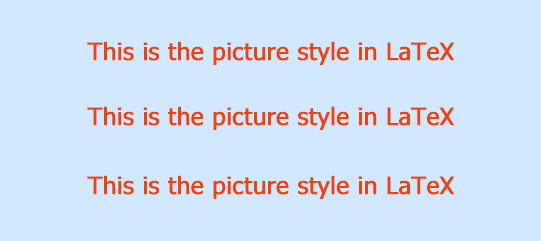
\includegraphics[scale=0.42]{picture-LaTeX.png}
\captionsetup{labelfont={bf},font={it,scriptsize}}
\caption{\scriptsize{\textit{This is the picture style in LaTeX}}}
\label{This is the picture style in $LaTeX$}
\end{figure}
\end{multicols}
\begin{table}[H]
\linespread{1.5}
\centering
\captionsetup{labelfont={bf},font={it,scriptsize}}
\caption{\scriptsize{\textit{This is the table style in LaTeX}}}
\scriptsize
\begin{tabular}{p{1.3cm}<{} p{1.3cm}<{} p{1.35cm}<{} p{1.4cm}<{} p{1.4cm}<{} p{1.4cm}<{} p{1.4cm}<{} p{1.4cm}<{} p{1.4cm}<{} p{1.4cm}<{}}
\bottomrule
\rowcolor{mygray}0 & 1 & 2 & 3 & 4 & 5 & 6 & 7 & 8 & 9  \\
\hline
\rowcolor{mygray}A=10& B=11 & C=12 & D=13 & E=14 & F=15 & G=16 & H=17 & J=18 & K=19 \\
\rowcolor{mygray}L=20 & M=21 & N=22 & P=23 & Q=24 & R=25 & S=26 & T=27 & U=28 & V=29 \\
\bottomrule
\end{tabular}
\end{table}
\begin{multicols}{2}
\section{SciencePG-Level1-Single-line}
The template will number citations consecutively within brackets [1] . The sentence punctuation follows the bracket [2]. Refer simply to the reference number, as in [3]¡ªdo not use ``Ref. [3]" or ``reference [3]" except at the beginning of a sentence: ``Reference [3] was the first . . ."

Number footnotes separately in superscripts. Place the actual footnote at the bottom of the column in which it was cited. Do not put footnotes in the reference list. Use letters for table footnotes.

Unless there are six authors or more give all authors' names; do not use ``et al.". Papers that have not been published, even if they have been submitted for publication, should be cited as ``unpublished" [4]. Papers that have been accepted for publication should be cited as ``in press" [5]. Capitalize only the first word in a paper title, except for proper nouns and element symbols.

For papers published in translation journals, please give the English citation first, followed by the original foreign-language citation [6].

If the square-shaped pixel size in our images was $8 \times 8$ screen-pixels, this amounted to about 21 pixels per face quantization (an equivalent of about 10.5 cycles/face). With this level of image detail, all three basic varieties of configural information (hange of spatial quantization between 11 pixels/face and 6 pixels/face levels altogether indicate that this ERP- component is especially sensitive to the first-order configural cues. Some other works have supported both of these ideas [6, 16, 25].

Unless there are six authors or more give all authors' names; do not use ``et al.". Papers that have not been published, even if they have been submitted for publication, should be cited as ``unpublished" [4]. Papers that have been accepted for publication should be cited as ``in press" [5]. Capitalize only the first word in a paper title, except for proper nouns and element symbols.

\section*{Acknowledgements}
The preferred spelling of the word `acknowledgment" in America is without an ``e" after the ``g". Avoid the stilted expression, ``One of us (R. B. G.) thanks . . ." Instead, try ``R. B. G. thanks". Put sponsor acknowledgments in the unnum-bered footnote on the first page.

\parskip=5pt
\noindent \rule[0pt]{25em}{1pt}

\parskip=10pt
\noindent {\References{Literaturverzeichnis}}
\vspace{-6pt}
\renewcommand{\bibsection}{}
\bibliographystyle{plainnat}
\bibliography{references}

\end{multicols}
\end{document}

